\section{Parallel Gradient Descent}
\label{ParGD}

Even with minibatches, the gradient computation can still be a bottleneck for most training algorithms.
There are two potential ways to get rid of this problem and we describe them in the subsequent subsections.

\subsection{Parallel Minibatch Gradient Descent}
\label{sub:PMGD}

Observe that the gradient is a sum of partial gradients with respect to the individual training examples.
So one way to parallelize gradient computation could be by distributing training examples of a minibatch across many processes, letting them compute a partial gradient over their own training examples and then summing up these partial gradients to get the approximate minibatch gradient.
This approach results in a procedure shown in algorithm \ref{alg:PMGD}.
\begin{algorithm}[tb]
   \caption{Parallel Minibatch Gradient Descent}
   \label{alg:PMGD}
\begin{algorithmic}
   \STATE {\bfseries Input:} Dataset $\mathcal{D} = \{x^{(i)},y^{(i)}\}_{i=1:N}$, Step Size $\alpha$, Max Epochs $N_{epoch}$, Batch Size $B$, Num Threads $T$
   \STATE {\bfseries Output:} Parameters $\{\theta_k\}_{k=1:K}$
   \STATE
   \STATE Initialize $\theta$ randomly with small real numbers
   \STATE $ep := 0$
   \REPEAT
   \STATE $ep := ep + 1$
   \STATE Divide $\mathcal{D}$ into batches $\{B_j\}_{j=1:\frac{N}{B}}$ of size $B$ each
   \FOR {$j \in \{1:\frac{N}{B}\}$}
   \STATE Divide $B_j$ into thread-batches $\{B_{jt}\}_{t=1:\frac{B}{T}}$ of size $\frac{B}{T}$
   \STATE \textbf{Thread `t' is forked:}
   \FOR {$k \in \{1:K\}$}
   \STATE $\frac{\partial \mathcal{L}_{MSE}}{\partial \theta_k} \big|_t := \sum_{i \in B_{jt}} ( y^{(i)} - f(x^{(i)}; \theta)) \frac{\partial f(x^{(i)}; \theta)}{\partial \theta_k}$
   \ENDFOR
   \STATE \textbf{Thread `t' joins back 'main'}
   \FOR {$k \in \{1:K\}$}
   \STATE $\frac{\partial \mathcal{L}_{MSE}}{\partial \theta_k} := \frac{1}{B} \sum_t \frac{\partial \mathcal{L}_{MSE}}{\partial \theta_k} \big|_t$
   \ENDFOR
   \STATE $\theta_k := \theta_k - \alpha \frac{\partial \mathcal{L}_{MSE}}{\partial \theta_k} \hspace{16pt} \forall k \in \{1:K\}$
   \ENDFOR
   \UNTIL{$ep \geq N_{epoch}$}
\end{algorithmic}
\end{algorithm}

\subsection{Parallelizing Matrix Computations}

An alternative way to parallelize the gradient computation process can be by parallelizing individual steps of backpropagation (algorithms \ref{alg:FwdPass} and \ref{alg:BackProp}).
Note that the forward propagation and backpropagation algorithms comprise various matrix vector multiplications which can be individually parallelized across multiple threads of execution.
Parallelized matrix-vector multiplications are already efficiently implemented in various linear algebra libraries and we will use the BLAS library to implement this second method of parallelization.

Graphics Processing Units (GPUs) are massively parallel processors that were designed for efficient computer graphics rendering and image processing. In fact, GPUs are very effective when used to execute the graphics rendering pipeline which is a sequence of geometric transformations on small multidimensional vectors. For this reason, GPUs are suitable for executing very fast certain linear algebra operations including but not limited to vector-vector addition, matrix-vector and matrix-matrix multiplication. Moreover, because GPUs consist of many throughput oriented multiprocessors that follow the Single Instruction Multiple Data (SIMD) execution model, they can be very useful for applications that require processing large amount of data.

\begin{figure}[ht]
%\vskip 0.2in
\begin{center}
\centerline{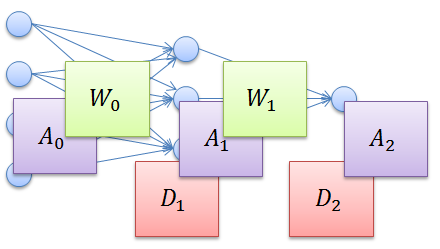
\includegraphics[width=\columnwidth]{gpu_neural_net_data}}
\caption{Abstract layered neural network architecture}
\label{fig:nn_architecture}
\end{center}
\vskip -0.2in
\end{figure}

Training neural networks is a process that can be realized through a series of matrix-matrix multiplications and additions which are applied for a large number of training examples. Every neural network can be defined and operated on by following this abstraction. Back propagation can be implemented as a series of kernel executions that are combined to ultimately compute the change in the weight values caused by the corresponding training batch. In our implementation, a neural network is viewed as a collection of layers, each one consisting of 3 distinct matrices. These matrices store the outgoing weight values $W_i$, the incoming activation values $A_i$ and the delta error values $D_i$ computed by back propagation. The activation values of the input layer (i.e. $A_0$) are the actual training examples in the corresponding batch. The activation values and the delta error values are stored in column-major order. In contrast the weights for each layer are stored in row-major order. The bias values are embedded in the last column of the weight matrix.

\begin{figure}[ht]
%\vskip 0.2in
\begin{center}
\centerline{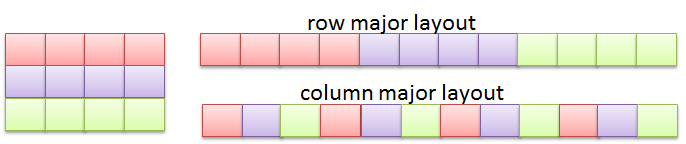
\includegraphics[width=\columnwidth]{gpu_data_layout}}
\caption{Matrix data layout}
\label{fig:data_layout}
\end{center}
\vskip -0.2in
\end{figure}

We decompose back-propagation into 5 steps each one implemented by distinct kernel. The first step, handles the feed forward activation by implementing a tiled matrix-matrix multiplication based on Eq.~\ref{act_kernel}. Here we denote with $f$ the preferred activation function which is usually the sigmoid function. Our implementation is designed around templates and supports user defined activation functions. The feed-forward step is implemented using the tiled matrix-matrix multiplication as it is described in CUDA samples. All threads participate in loading the tiles of the input matrices into shared memory. The threads use registers to accumulate partial results. After parsing the complete matrix each thread applies the activation function on the resulting value before storing it into global memory. All read and write operations to global memory are coalesced and there are no bank conflicts because thread iterate over the secondary matrix dimension in each case. An additional step is required to initialize the thread registers with the bias values.

\begin{equation}\label{act_kernel}
A_{i+1} = f\left(W_{i} \cdot A_{i} + b_i\right), \forall i \in \left[1,L-1\right]
\end{equation}

\begin{equation}\delta_output_kernel
D_{L} = Y - A_{L}
\end{equation}

\begin{equation}\label{delta_kernel}
D_{i} = W_{i}^T \cdot D_{i} \circ d(W_{i-1} \cdot A_{i+1})
\end{equation}

\begin{equation}\label{update_kernel}
W_{i} = W_{i} + \frac{n}{b} \cdot \sum_{j=1}^{b} D_{i+1}^{j} \cdot (A_{i}^j)^T
\end{equation}

Following this previous step, the delta error values are computed for each layer using Eq.~\ref{delta_kernel}. This equation is computed using 3 kernels, one for computing the output layer delta and two more that compute the transpose matrix-matrix multiplication and the hadamard product of the derivative for the corresponding activation function. A variation of the tiled matrix-matrix multiplication kernel is used to perform these operations. For the first kernel, the indexing is changed to enable multiplication with the transpose of the weight matrix. Here accesses to global memory remain coalesced since we order the thread blocks vertically on the weight matrix. However, we incur few bank conflicts when accessing the data in column-major order from shared-memory . In the second case, we chose to re-compute the product of $W_i \cdot A_i$ and multiply it with the result from the previous operation. This is because are goal was to support arbitrary defined activation functions. In case the sigmoid function is used, the derivative can be replaced with $A_i \cdot \left(1.0 - A_i\right)$ which enables significant reduction of the required computation.

Finally, we use the computed activation and the next layer delta matrices (Eq.~\ref{update_kernel}) to update the weights of the corresponding layer depending on the chosen learning rate and batch size. This operation can be considered as another variation of matrix-matrix multiplication where each column from $ D_{i+1}$ and $A_{i}$ are  multiplied to produced a single matrix. The number of resulting matrices are equal to the batch size and are accumulated in thread registers. The resulting summation is multiplied by $\frac{n}{b}$ and added to the weight values of the corresponding layer. For this operation, access to global memory is again coalesced. However, shared memory access incurs many bank conflicts which are proportional to the batch size. In order to improve the performance, the corresponding tiles are loaded transposed into shared memory. This incurs only a single bank conflict during loading and avoids many bank conflicts during the multiplication phase.